\documentclass[30pt]{tikzposter}

% design based on https://twitter.com/mikemorrison/status/1110191245035479041?lang=en
% and https://github.com/SimonLarsen/tikzpostersdu

\usepackage{tikzposterSDU}
\usepackage{bm}
\usepackage{amsfonts}       % blackboard math symbols
\usepackage{amsmath}
\usepackage[bitstream-charter]{mathdesign}
\usepackage[scaled=0.9,sfdefault]{FiraSans}

% set page dimensions
\geometry{paperwidth=100cm, paperheight=70cm}
\makeatletter
\setlength{\TP@visibletextwidth}{\textwidth-2\TP@innermargin}
\setlength{\TP@visibletextheight}{\textheight-2\TP@innermargin}
\makeatother

\usetheme{SDU}

% background color
\colorlet{blockbodybgcolor}{white}
\colorlet{backgroundcolor}{mDarkTeal}


\newcommand{\Wre}{ W_{r}}
\newcommand{\Wim}{ W_{i}}

\newcommand{\nobackgroundblock}[1]{
  \colorlet{blockbodybgcolor}{mDarkTeal}
    \block{}{\color{white}{#1}}
  \colorlet{blockbodybgcolor}{white}
}

\tikzposterlatexaffectionproofoff


\hyphenation{RealNPU}

\begin{document}

% remove offset that would otherwise be fixed by \maketitle
\makeatletter
\setlength{\TP@blocktop}{.47\textheight}
\makeatother

\begin{columns}

  \column{0.53}
    \nobackgroundblock{
      {\fontseries{l}\fontsize{60}{80}\selectfont
        \textbf{\emph{Neural Power Units}} -
        Learning to \textbf{extrapolate} functions composed of
        \textbf{arithmetic operations}.
      }
    }

  \column{0.17}
    \nobackgroundblock{
      \begin{center}
        {\fontseries{l}\fontsize{35}{40}\selectfont
          Niklas Heim\\
          V\'aclav \v Sm\'idl\\
          Tom\'a\v s Pevn\'y}
      \end{center}
    }

  \column{0.30}
  \block{}{
    \begin{minipage}{0.18\textwidth}
      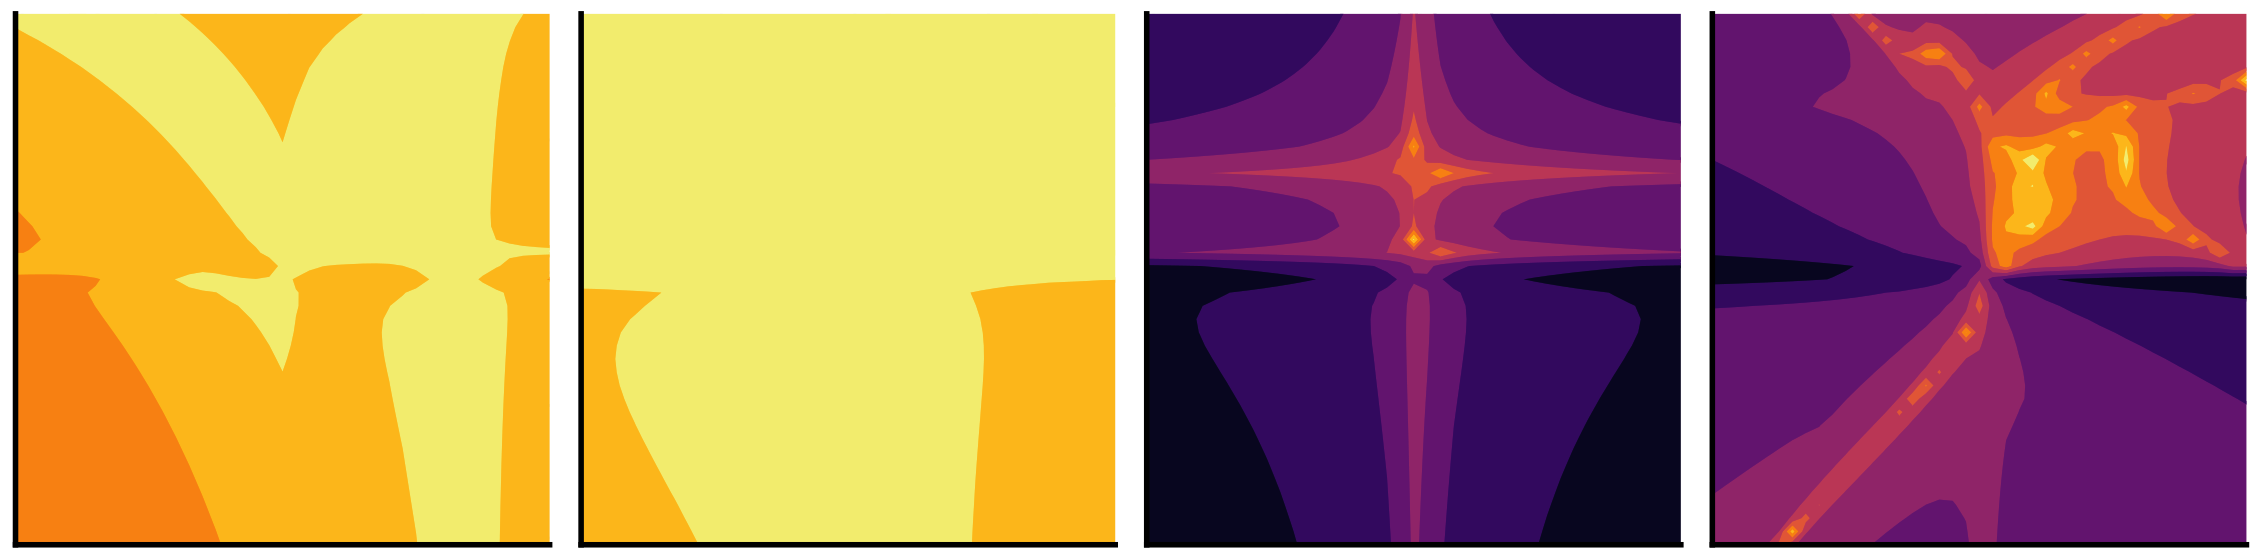
\includegraphics[width=\textwidth]{div-logo.png}
    \end{minipage}
    \hfill
    \begin{minipage}{0.08\textwidth}
      \begin{flushleft}
      Czech Technical University\\
      Prague
      \end{flushleft}
    \end{minipage}
  }

\end{columns}


\begin{columns}

  \column{0.53}
  \block{}{
    \centering
    \begin{minipage}{0.1\textwidth}
      \centering
      \textbf{Neural Power Unit}\\
      schematic with the \textbf{relevance gate}\\
      shaded in grey
    \end{minipage}
    \hspace{2cm}
    \begin{minipage}{0.33\columnwidth}
      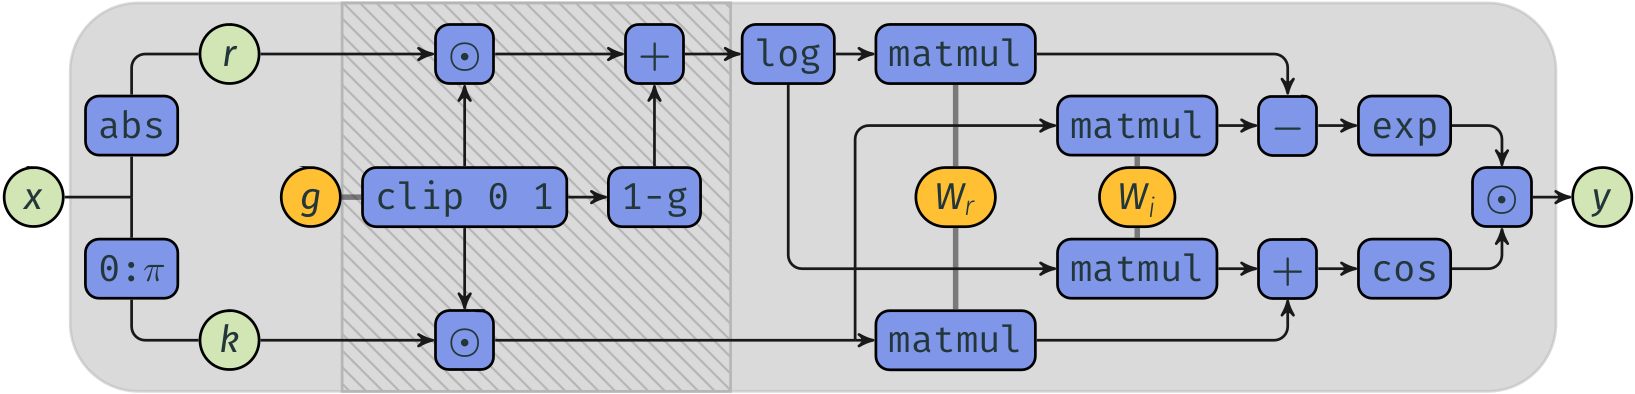
\includegraphics[width=\textwidth]{npu.png}
    \end{minipage}
  }


  \begin{subcolumns}
    \subcolumn{0.5}
    \block{Neural Arithmetic}{
      \emph{Neural Arithmetic} (or \emph{Arithmetic Extrapolation}) uses
      inductive biases to increase the extrapolation performance of neural
      networks on tasks in which the underlying function is \emph{partially}
      composed of arithmetic operations.
    }
    \block{Neural Power Unit (NPU)}{
      The NPU (inspired by NALU; Trask et al.) uses complex arithmetic to correctly
      process negative numbers and contains a relevance gate $g$ for
      more consistent convergence and sparser solutions.
      \begin{align*}
        y &= \exp(\Wre \log r - \pi\Wim k) \\
          &\odot \cos(\Wim\log  r + \pi\Wre k),
      \end{align*}
      where
      \begin{align*}
        \label{eq:gatednpu_def}
        r &= {\hat g} \odot (| x|+\epsilon) + (1-{\hat g}), \\
        k_i &= \begin{cases}
           0  & x_i \geq 0 \\
          \hat g_i & x_i < 0
        \end{cases},\\
        \hat g_i &= \min(\max(g_i,0),1),
      \end{align*}
      with inputs $ x$, and trainable parameters $\Wre$, $\Wim$, $g$.\\
      In the \textbf{RealNPU} we fix $\Wim$ to zero to
      obtain a highly transparent model.
    }

    \block{Prior art}{
      \begin{itemize}
        \item \emph{NALU} (Trask et al.): Can perform $(+,\times,\div)$,
          but cannot handle negative numbers and has convergence problems.
        \item \emph{NMU \& NAU} (Madsen \& Johansen): Can perform addition and multiplication,
          but no division.
      \end{itemize}
    }

    \subcolumn{0.5}
    \block{Our Contributions}{
      \begin{itemize}
        \item Learning \textbf{multiplication}, \textbf{division} and
          fractional \textbf{power functions} 
        \item Correct processing of \textbf{negative inputs}  
        \item \textbf{Relevance gating} for reliable convergence and sparse solutions
        \item A \textbf{transparent} model for applications like equation discovery (RealNPU)
      \end{itemize}
    }

    \block{Relevance gate}{
      On a toy task of learning $f(x,y) = x$ we demonstrate that
      the \emph{NaiveNPU} (without the relevance gate) has a zero gradient norm
      in large parts of parameter space (left plot).
      In the NPU (with the gate) the gradient surface becomes much more informative.
      \vspace{1cm}

      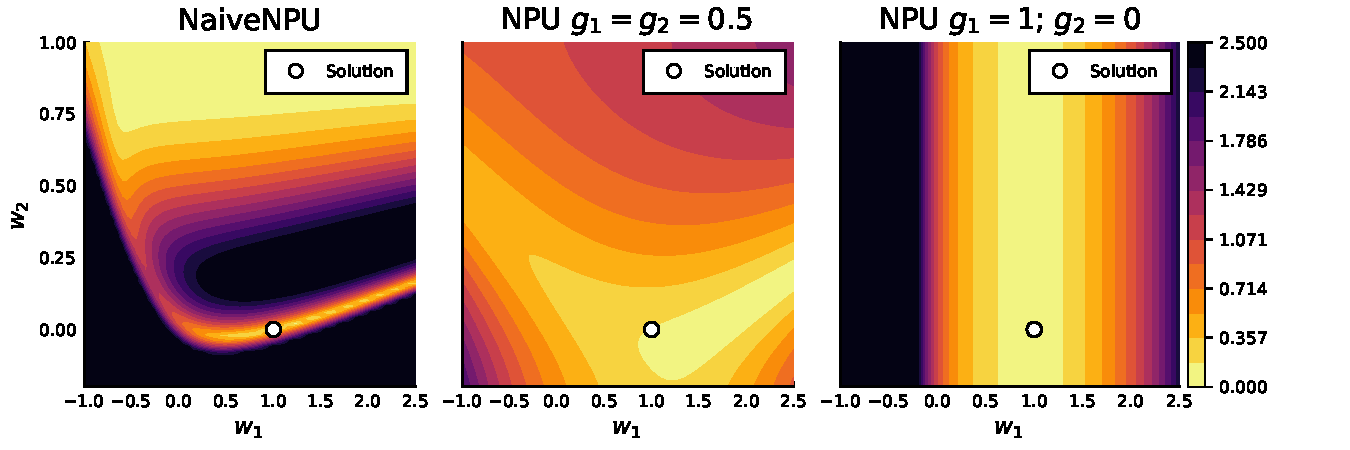
\includegraphics[width=0.235\textwidth]{../plots/npu_gatednpu_id_grad.pdf}
    }
    \block{}{
      Find all the details in our paper or contact us via
      \texttt{heimnikl@fel.cvut.cz}.

      \vspace{1.5cm}
      \begin{center}
        \begin{minipage}{0.07\textwidth}
          \centering
          Paper\\
          \vspace{0.3cm}
          
\includegraphics[height=4.5cm]{qr-paper.png}
        \end{minipage}
        \hspace{2cm}
        \begin{minipage}{0.07\textwidth}
          \centering
          Code\\
          \vspace{0.3cm}
          
\includegraphics[height=4.5cm]{qr-code.png}
        \end{minipage}
      \end{center}
      \vspace{1.05cm}
    }
  \end{subcolumns}


  \column{0.47}
  \block{Extrapolation experiment}{
    %\begin{multicols}{2}
      Prediction error for different models trained to learn $f$ on training
      samples $(x,y) \sim U(0.01,2)$.
      \begin{equation*}
        f(x,y) = (x+y,\, xy,\, \frac{x}{y},\, \sqrt{x} \text{  })^T
      \end{equation*}
      Bright colors indicate low error. All models learn the problem within the
      training range, but only the NPU manages to learn all operations including
      the fractional power $\sqrt{x}$.
    %\end{multicols}
    \begin{center}
      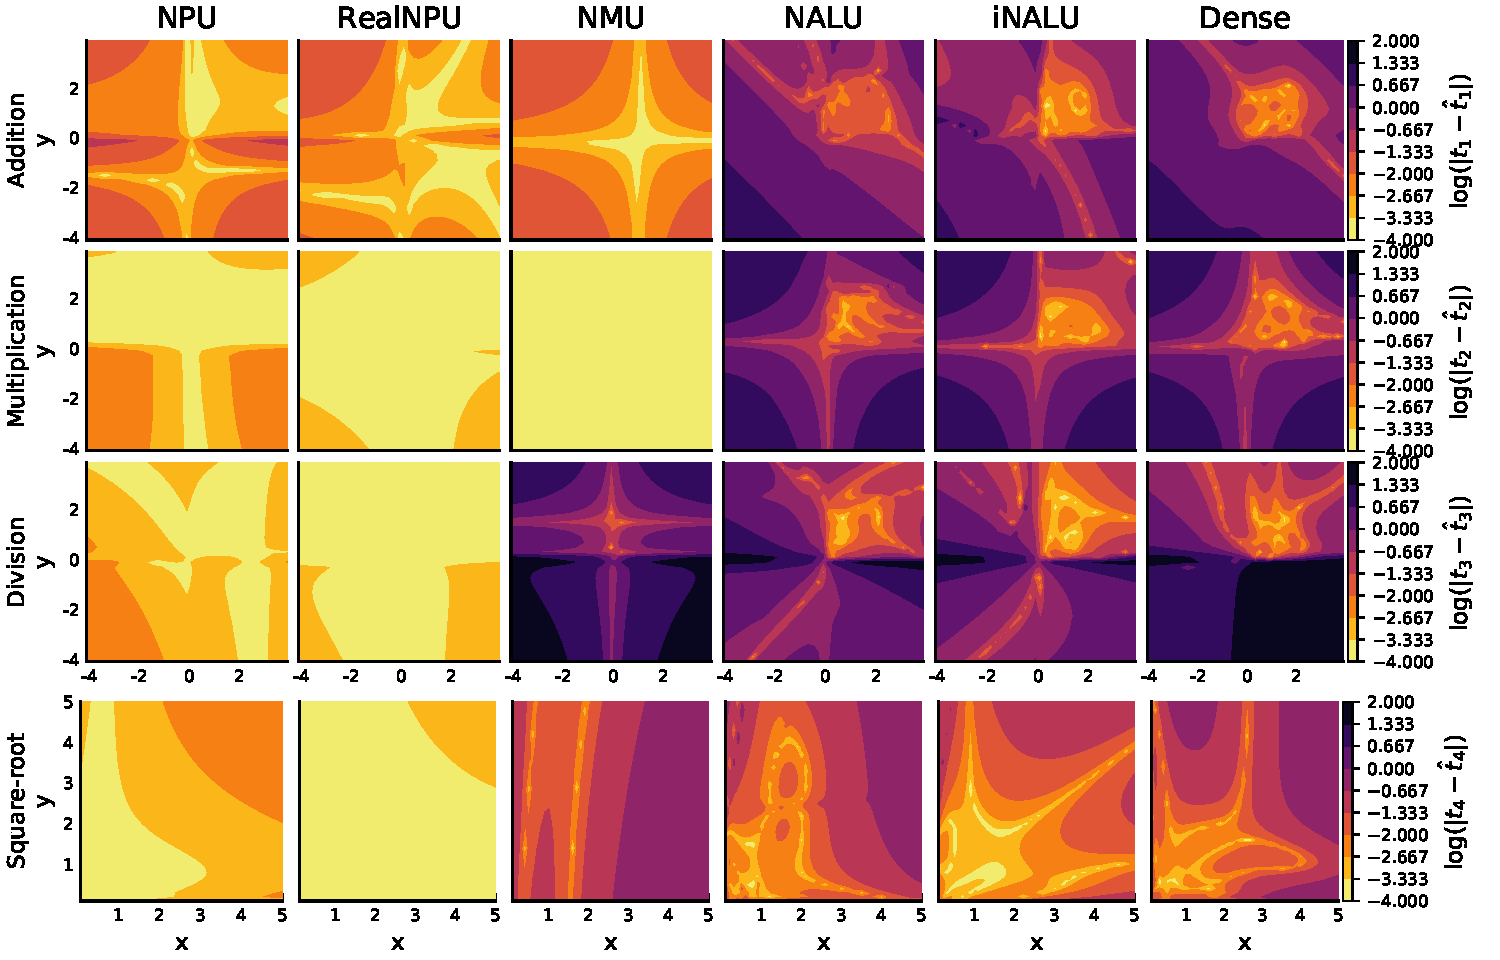
\includegraphics[width=0.4\textwidth]{../plots/simple_err.pdf}
    \end{center}
  }
  \block{Towards Equation Discovery}{
    %\begin{multicols}{2}
      Our paper sketches how to use the \textbf{RealNPU} for equation discovery
      of ODEs with fractional powers.  The RealNPU (Layer 1) on the right
      discovers a product of fractional powers in the first row of weights.
      The NAU (Layer 2) looks very similar to the parameter matrix of the
      \emph{fSIR} model (Taghvaei et al.) on the left.
    %\end{multicols}

    \begin{center}
      \begin{minipage}{.14\textwidth}
        \begin{equation*}
          \begin{bmatrix}
            \dot S \\ \dot I \\ \dot R
          \end{bmatrix}
          =
          \begin{bmatrix}
            \text{-}\beta & 0 & \eta \\
            \beta & \text{-}\alpha & 0 \\
            0 & \alpha & \eta
          \end{bmatrix}
          \begin{bmatrix}
            I^\gamma S^\kappa \\ I \\ R
          \end{bmatrix}
        \end{equation*}
      \end{minipage}
      \hspace{2cm}
      \begin{minipage}{.25\textwidth}
        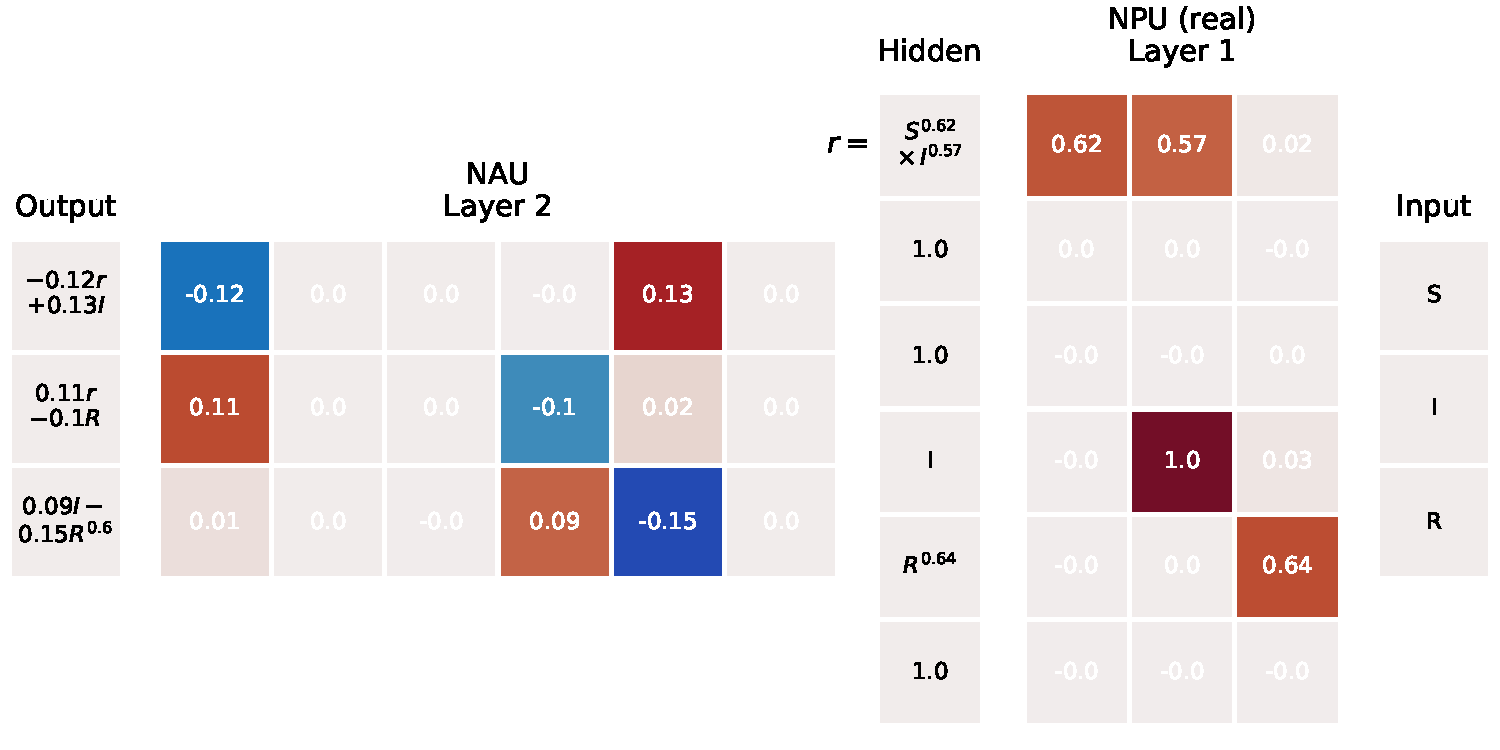
\includegraphics[width=\textwidth]{../plots/sir_gatednpu_modelps.pdf}
      \end{minipage}
    \end{center}
    \vspace{0.5cm}
  }


\end{columns}

\end{document}
